\begin{tikzpicture}
    \node[diagram/histogram card] (pequena) at (0,0) {};
    \node[diagram/histogram card] (intermedia) at (5.5,0) {};
    \node[diagram/histogram card] (grande) at (11,0) {};

    \node[diagram/card title] at (0,2.75) {MUESTRA PEQUEÑA};
    \node[diagram/card title] at (5.5,2.75) {MUESTRA INTERMEDIA};
    \node[diagram/card title] at (11,2.75) {MUESTRA GRANDE};

    \node[inner sep=0pt] at (0,0.05)
        {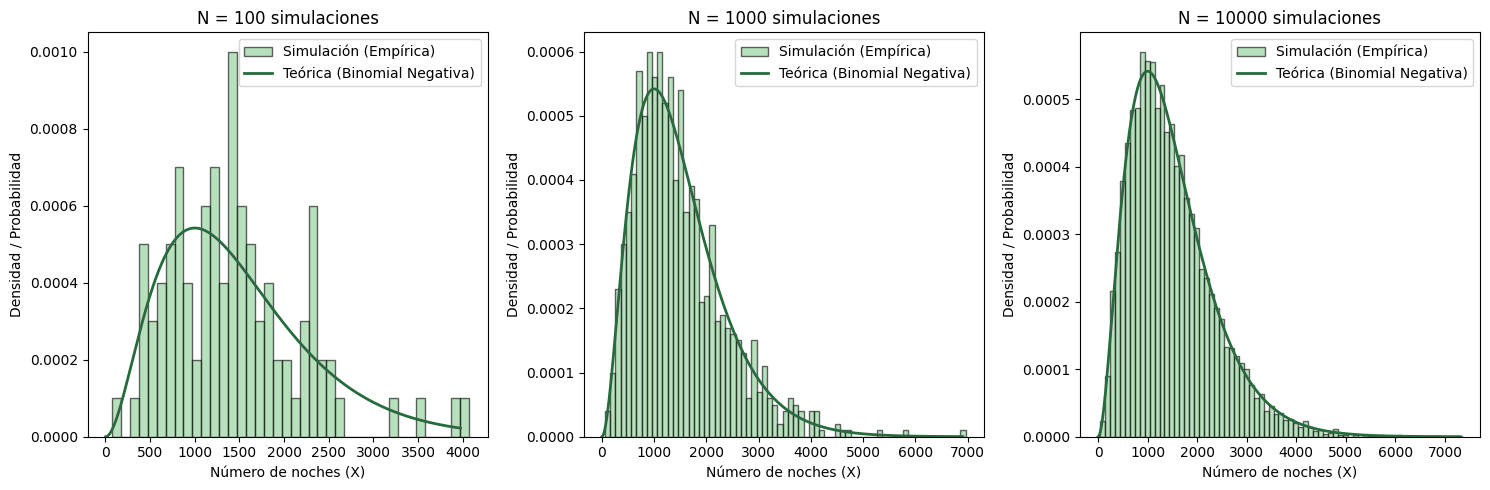
\includegraphics[width=4.9cm,trim={0bp 0bp 712.8bp 0bp},clip]
            {figuras/histogramas.png}};
    \node[inner sep=0pt] at (5.5,0.05)
        {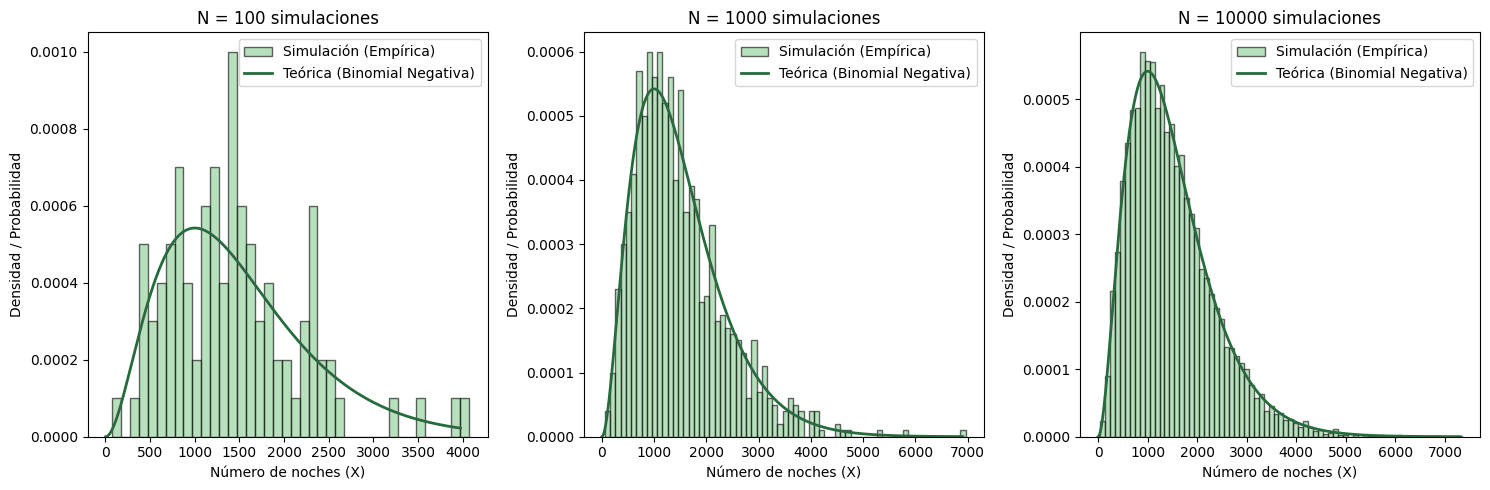
\includegraphics[width=4.9cm,trim={360bp 0bp 360bp 0bp},clip]
            {figuras/histogramas.png}};
    \node[inner sep=0pt] at (11,0.05)
        {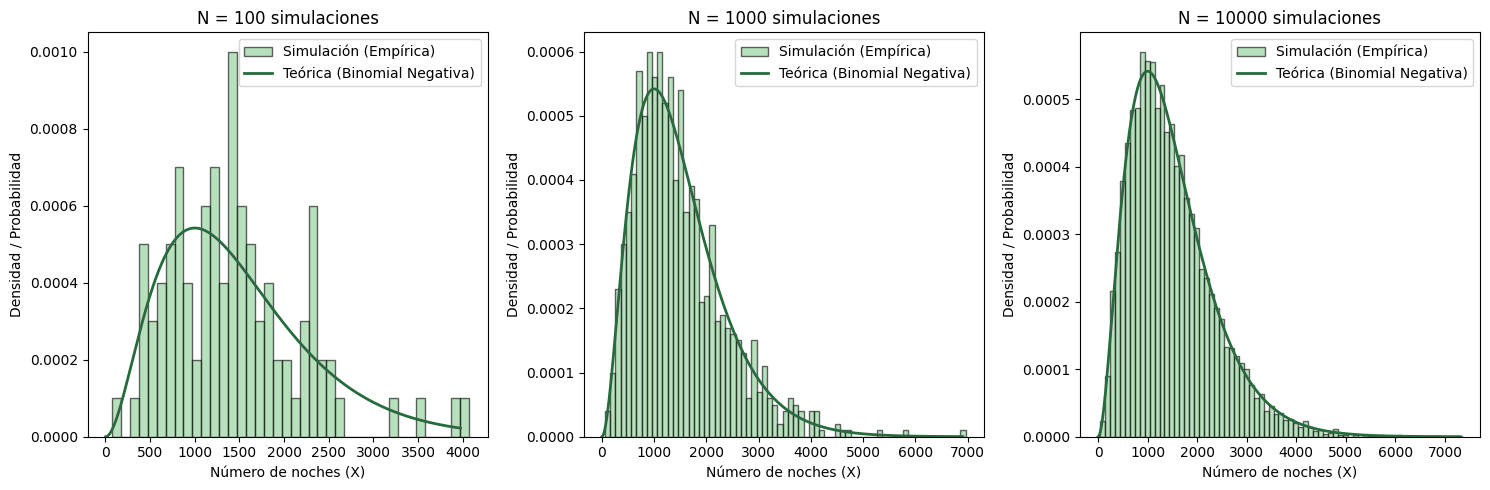
\includegraphics[width=4.9cm,trim={712.8bp 0bp 0bp 0bp},clip]
            {figuras/histogramas.png}};

    \node[diagram/card note] at (0,-2.8) {Alta variabilidad};
    \node[diagram/card note] at (5.5,-2.8) {Menores fluctuaciones};
    \node[diagram/card note] at (11,-2.8) {Mayor acuerdo visual};

    \draw[diagram/arrow, draw=diagramTeal, line width=1.2pt]
        (0,-3.65) -- (11,-3.65);
    \node[diagram/edge label, font=\small\bfseries,
          text=diagramTeal] at (5.5,-3.65)
        {Aumento del número de simulaciones};
    \node[align=center, font=\small, text=diagramInk,
          text width=15cm] at (5.5,-4.4)
        {La distribución empírica se aproxima a la teórica\\
         y el ruido muestral se reduce.};
\end{tikzpicture}